\documentclass{article}

\usepackage[numbers]{natbib}
\usepackage{hyperref}
\usepackage{graphicx}

\title{$z$-score normalized cumulative rain-use efficiency differences over the Kilimanjaro region}
\author{Florian Detsch (florian.detsch@staff.uni-marburg.de)}
\date{December 11, 2015}

\begin{document}

\maketitle

The herein presented data is heavily based on the study by \citet{Landmann2014} who investigated land degradation over East Africa on the basis of $z$-score normalized cumulative rain-use efficiency differences (\textit{CRD}). In order to assess area-wide CRD, the authors used monthly rain-use efficiencies (\textit{RUE}; \cite{Prince1998a}) calculated from 

\begin{equation}
\label{rue}
\textit{RUE} = \frac{P_n}{P_r}
\end{equation}

where $P_n$ and $P_r$ are monthly estimates of net primary productivity (\textit{NPP}) and precipitation, respectively. $z$-score normalized CRD was then calculated from 

\begin{equation}
\textit{CRD} = \sum \limits_{i=1}^n \textit{RUE}_{y_{i+1}} - \textit{RUE}_{y_{i}}
\end{equation}

where $\textit{RUE}_{y_{i}}$ means the value of RUE in year $y_{i}$ as derived from Equation \ref{rue}, and $n$ is the number of years under investigation. Accordingly, the processing chain used to derive area-wide CRD over the Kilimanjaro region, Tanzania, includes the following work steps:

\begin{itemize}
\item Monthly maximum value composites (MVC) of the Normalized Difference Vegetation Index \citep[NDVI;][]{Tucker1979} are created from the 16-day products originating from the Moderate Resolution Imaging Spectroradiometers (MODIS) aboard NASA's Terra and Aqua satellites. These are 'deseasoned', i.e. intra-annual seasonal fluctuations originating from the bimodal annual rainfall distribution \citep{Otte2015} are removed by subtracting the long-term monthly means from the respective raw values \citep{Appelhans2015b}, and subsequently used to calculate 'conclusive' \cite[$p<0.001$;][]{Miller1966} long-term trends (Figure 1).

\item Monthly $P_n$ is derived from fitting pixel-based linear models to annual MODIS estimates of NDVI and NPP. The models are subsequently used to predict monthly NPP on the basis of monthly raw NDVI.

\item Monthly $P_r$ is derived from the 5-km Climate Hazards Group InfraRed Precipitation with Station data (CHIRPS; \citep{Funk2015}). 

\item Monthly values of RUE and, finally, area-wide estimates of the CRD (shown in Figure 2 for all 'conclusive' Aqua-MODIS-based linear trends as depicted in Figure 1b) are calculated from the thus derived estimates of $P_n$ and $P_r$. 
\end{itemize}


%%% figure 1, trends
\begin{figure}[!htbp]
\label{fig_trends}
	\begin{center}
		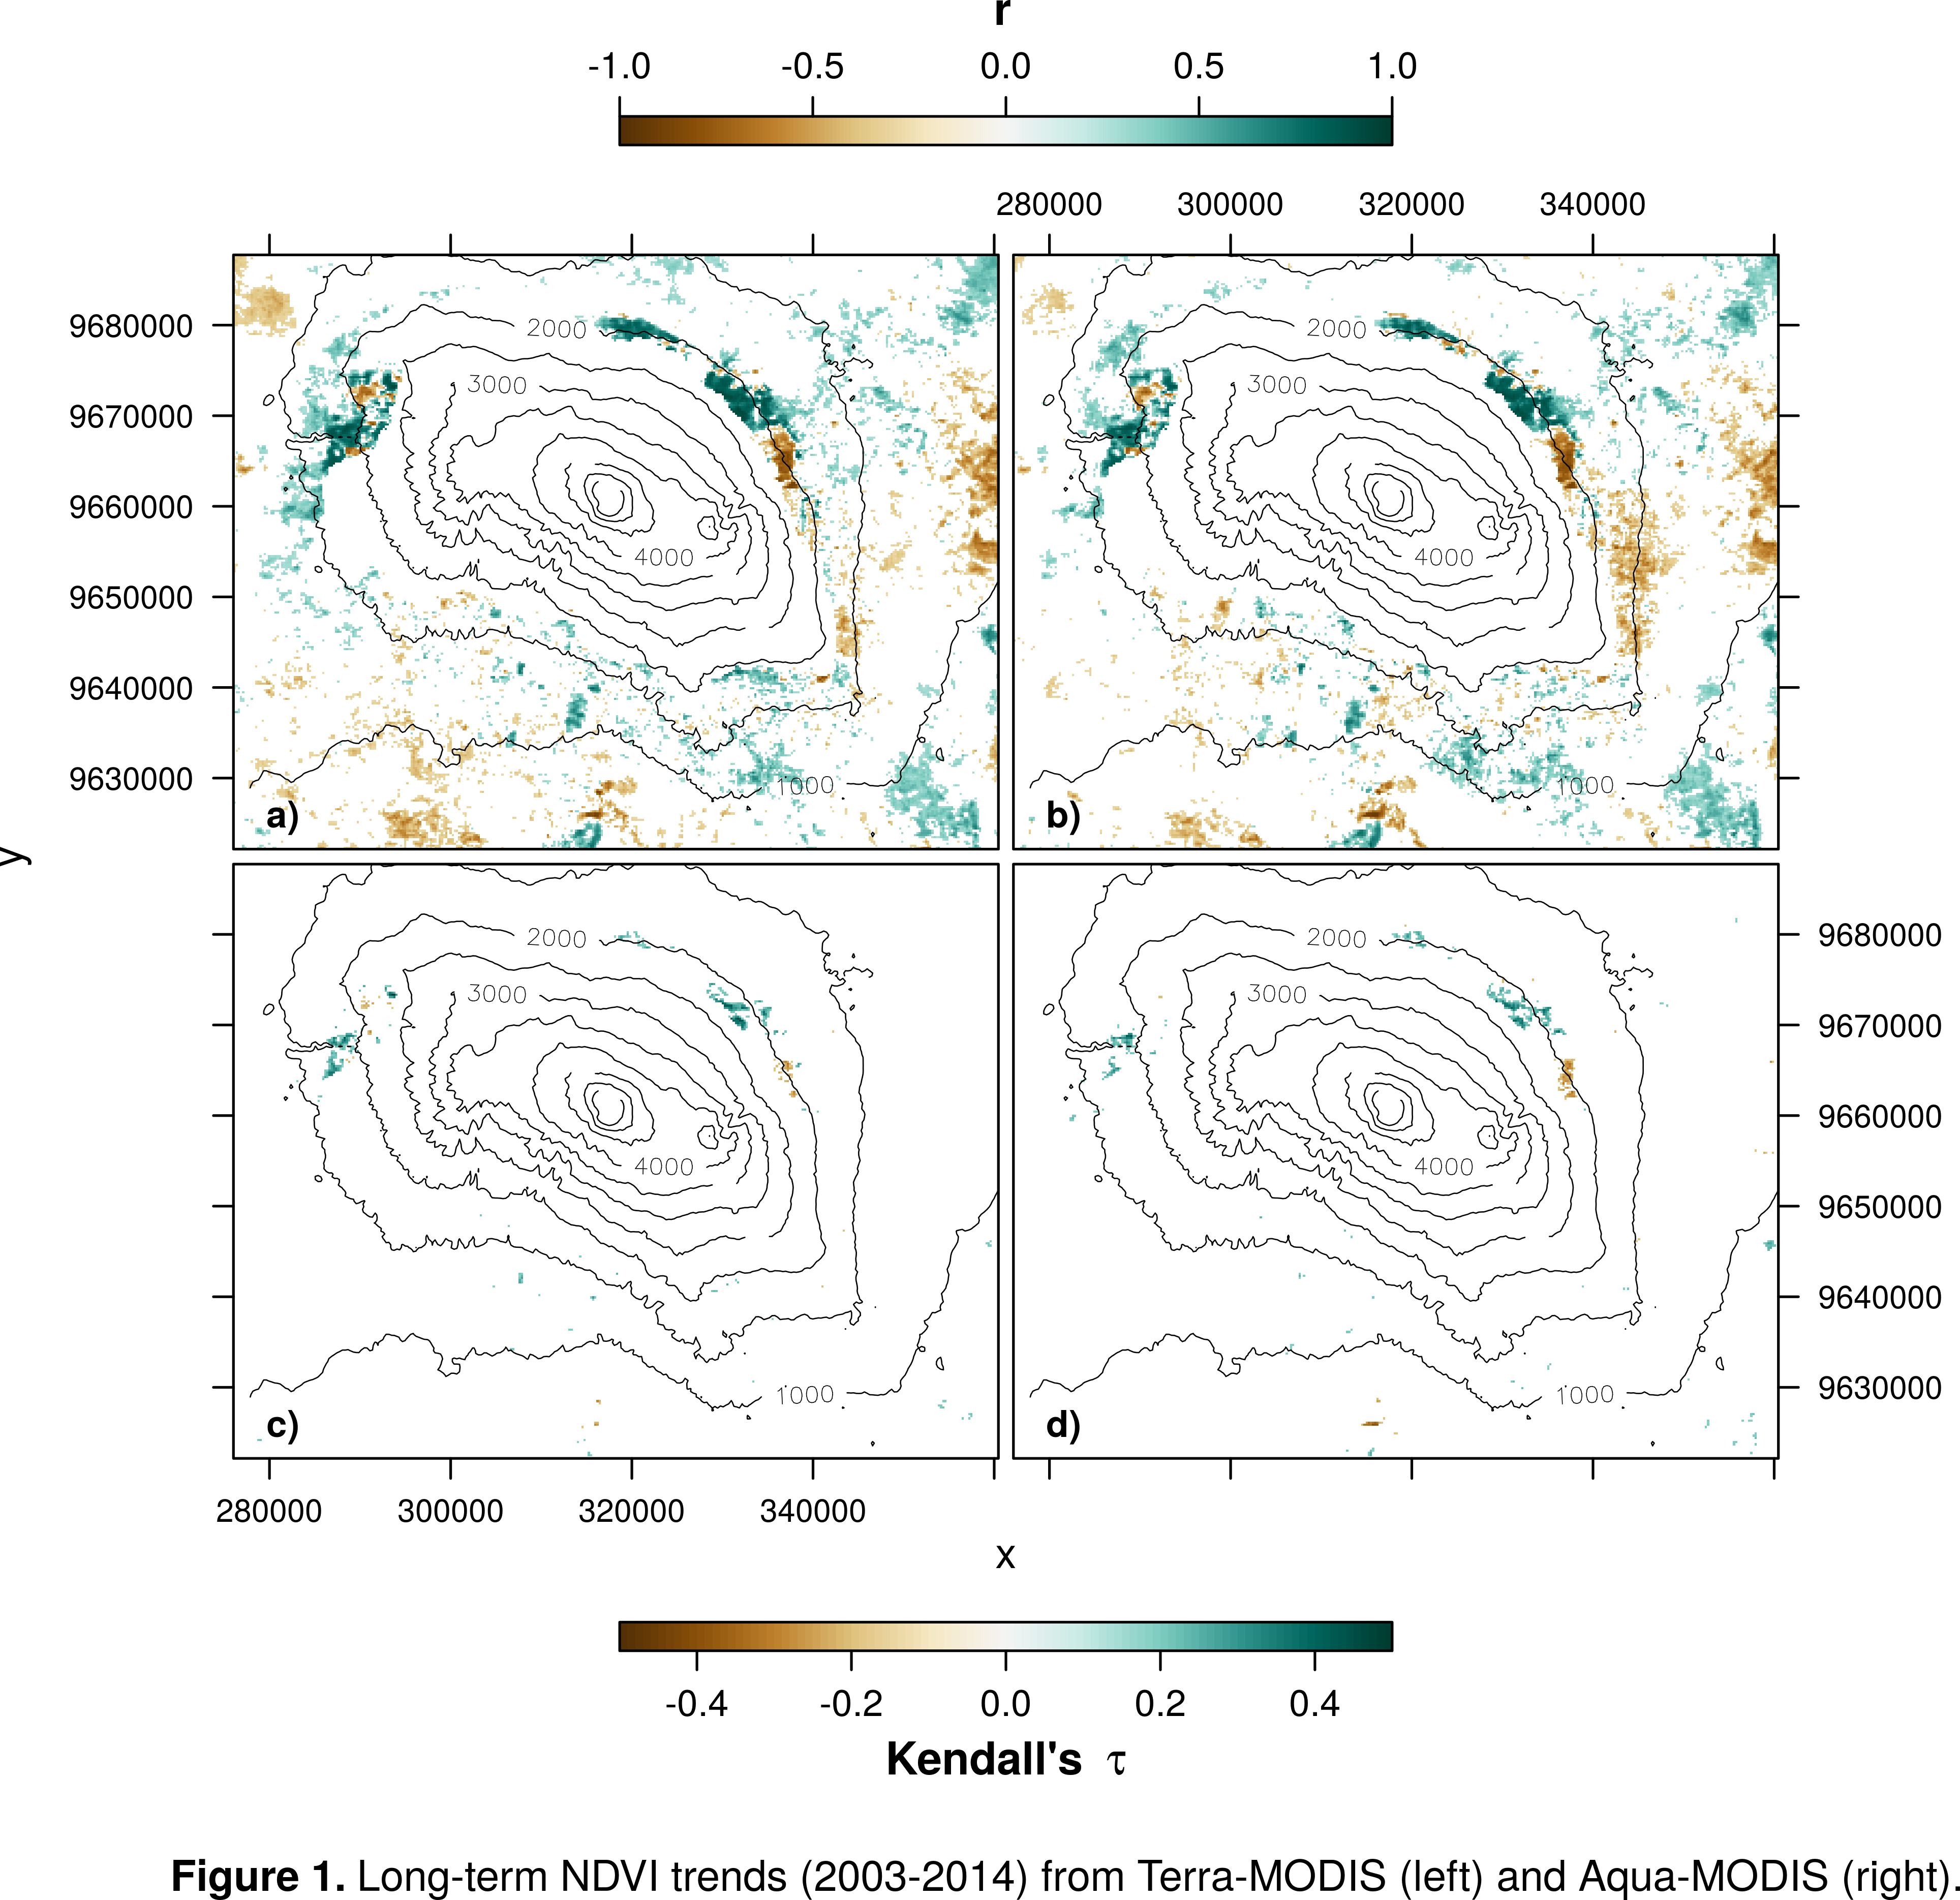
\includegraphics[width = 1\textwidth]{img/figure_trends.png}
	\end{center}
\end{figure}
 
%%% figure 2, crd 
\begin{figure}[!htbp]
\label{fig_crd}
	\begin{center}
		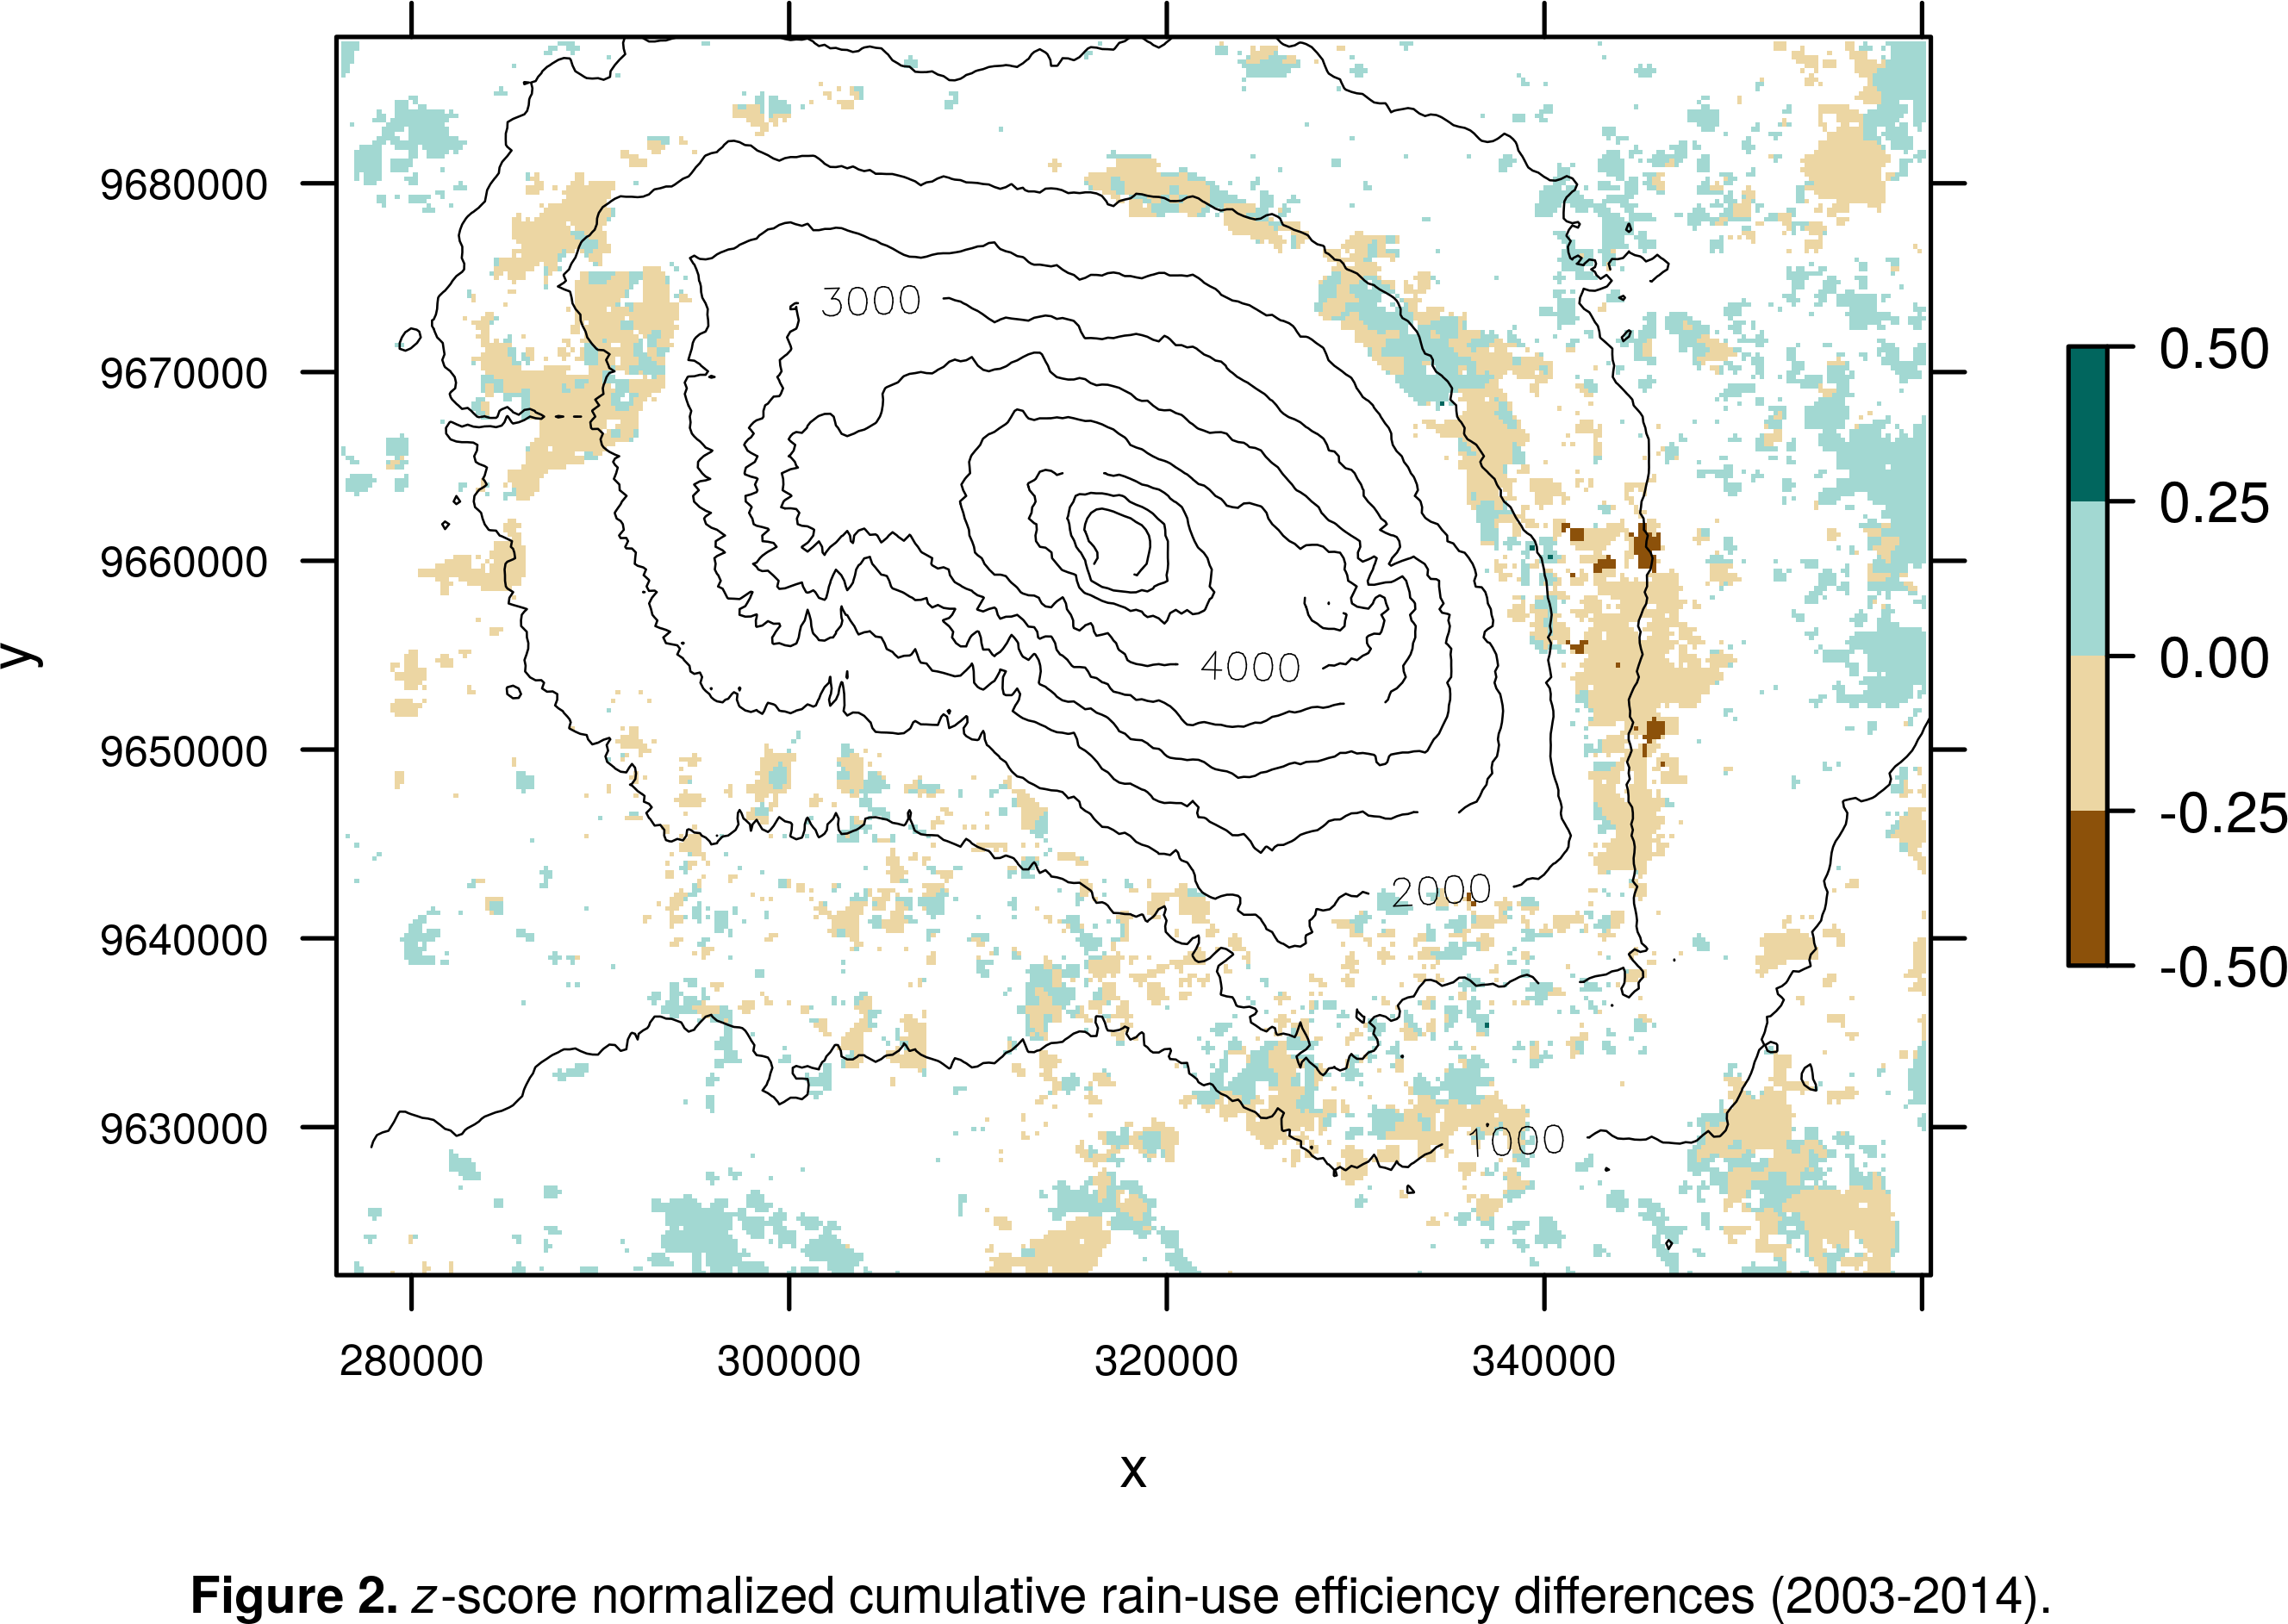
\includegraphics[width = 1\textwidth]{img/figure_crd.png}
	\end{center}
\end{figure}
 
 
\clearpage  
\bibliographystyle{mdpi}
\bibliography{readme}

\end{document}

